% GNUPLOT: LaTeX picture with Postscript
\begingroup
  \makeatletter
  \providecommand\color[2][]{%
    \GenericError{(gnuplot) \space\space\space\@spaces}{%
      Package color not loaded in conjunction with
      terminal option `colourtext'%
    }{See the gnuplot documentation for explanation.%
    }{Either use 'blacktext' in gnuplot or load the package
      color.sty in LaTeX.}%
    \renewcommand\color[2][]{}%
  }%
  \providecommand\includegraphics[2][]{%
    \GenericError{(gnuplot) \space\space\space\@spaces}{%
      Package graphicx or graphics not loaded%
    }{See the gnuplot documentation for explanation.%
    }{The gnuplot epslatex terminal needs graphicx.sty or graphics.sty.}%
    \renewcommand\includegraphics[2][]{}%
  }%
  \providecommand\rotatebox[2]{#2}%
  \@ifundefined{ifGPcolor}{%
    \newif\ifGPcolor
    \GPcolortrue
  }{}%
  \@ifundefined{ifGPblacktext}{%
    \newif\ifGPblacktext
    \GPblacktexttrue
  }{}%
  % define a \g@addto@macro without @ in the name:
  \let\gplgaddtomacro\g@addto@macro
  % define empty templates for all commands taking text:
  \gdef\gplbacktext{}%
  \gdef\gplfronttext{}%
  \makeatother
  \ifGPblacktext
    % no textcolor at all
    \def\colorrgb#1{}%
    \def\colorgray#1{}%
  \else
    % gray or color?
    \ifGPcolor
      \def\colorrgb#1{\color[rgb]{#1}}%
      \def\colorgray#1{\color[gray]{#1}}%
      \expandafter\def\csname LTw\endcsname{\color{white}}%
      \expandafter\def\csname LTb\endcsname{\color{black}}%
      \expandafter\def\csname LTa\endcsname{\color{black}}%
      \expandafter\def\csname LT0\endcsname{\color[rgb]{1,0,0}}%
      \expandafter\def\csname LT1\endcsname{\color[rgb]{0,1,0}}%
      \expandafter\def\csname LT2\endcsname{\color[rgb]{0,0,1}}%
      \expandafter\def\csname LT3\endcsname{\color[rgb]{1,0,1}}%
      \expandafter\def\csname LT4\endcsname{\color[rgb]{0,1,1}}%
      \expandafter\def\csname LT5\endcsname{\color[rgb]{1,1,0}}%
      \expandafter\def\csname LT6\endcsname{\color[rgb]{0,0,0}}%
      \expandafter\def\csname LT7\endcsname{\color[rgb]{1,0.3,0}}%
      \expandafter\def\csname LT8\endcsname{\color[rgb]{0.5,0.5,0.5}}%
    \else
      % gray
      \def\colorrgb#1{\color{black}}%
      \def\colorgray#1{\color[gray]{#1}}%
      \expandafter\def\csname LTw\endcsname{\color{white}}%
      \expandafter\def\csname LTb\endcsname{\color{black}}%
      \expandafter\def\csname LTa\endcsname{\color{black}}%
      \expandafter\def\csname LT0\endcsname{\color{black}}%
      \expandafter\def\csname LT1\endcsname{\color{black}}%
      \expandafter\def\csname LT2\endcsname{\color{black}}%
      \expandafter\def\csname LT3\endcsname{\color{black}}%
      \expandafter\def\csname LT4\endcsname{\color{black}}%
      \expandafter\def\csname LT5\endcsname{\color{black}}%
      \expandafter\def\csname LT6\endcsname{\color{black}}%
      \expandafter\def\csname LT7\endcsname{\color{black}}%
      \expandafter\def\csname LT8\endcsname{\color{black}}%
    \fi
  \fi
    \setlength{\unitlength}{0.0500bp}%
    \ifx\gptboxheight\undefined%
      \newlength{\gptboxheight}%
      \newlength{\gptboxwidth}%
      \newsavebox{\gptboxtext}%
    \fi%
    \setlength{\fboxrule}{0.5pt}%
    \setlength{\fboxsep}{1pt}%
\begin{picture}(9620.00,9620.00)%
    \gplgaddtomacro\gplbacktext{%
      \csname LTb\endcsname%
      \put(603,5057){\makebox(0,0)[r]{\strut{}$0$}}%
      \csname LTb\endcsname%
      \put(603,5429){\makebox(0,0)[r]{\strut{}$2$}}%
      \csname LTb\endcsname%
      \put(603,5801){\makebox(0,0)[r]{\strut{}$4$}}%
      \csname LTb\endcsname%
      \put(603,6172){\makebox(0,0)[r]{\strut{}$6$}}%
      \csname LTb\endcsname%
      \put(603,6544){\makebox(0,0)[r]{\strut{}$8$}}%
      \csname LTb\endcsname%
      \put(603,6916){\makebox(0,0)[r]{\strut{}$10$}}%
      \csname LTb\endcsname%
      \put(603,7288){\makebox(0,0)[r]{\strut{}$12$}}%
      \csname LTb\endcsname%
      \put(603,7660){\makebox(0,0)[r]{\strut{}$14$}}%
      \csname LTb\endcsname%
      \put(603,8031){\makebox(0,0)[r]{\strut{}$16$}}%
      \csname LTb\endcsname%
      \put(603,8403){\makebox(0,0)[r]{\strut{}$18$}}%
      \csname LTb\endcsname%
      \put(603,8775){\makebox(0,0)[r]{\strut{}$20$}}%
      \csname LTb\endcsname%
      \put(956,4858){\makebox(0,0){\strut{}$2$}}%
      \csname LTb\endcsname%
      \put(1486,4858){\makebox(0,0){\strut{}$4$}}%
      \csname LTb\endcsname%
      \put(2017,4858){\makebox(0,0){\strut{}$6$}}%
      \csname LTb\endcsname%
      \put(2547,4858){\makebox(0,0){\strut{}$8$}}%
      \csname LTb\endcsname%
      \put(3077,4858){\makebox(0,0){\strut{}$10$}}%
      \csname LTb\endcsname%
      \put(3607,4858){\makebox(0,0){\strut{}$12$}}%
      \csname LTb\endcsname%
      \put(4138,4858){\makebox(0,0){\strut{}$14$}}%
      \csname LTb\endcsname%
      \put(4668,4858){\makebox(0,0){\strut{}$16$}}%
      \csname LTb\endcsname%
      \put(4756,5057){\makebox(0,0)[l]{\strut{} }}%
      \csname LTb\endcsname%
      \put(4756,5429){\makebox(0,0)[l]{\strut{} }}%
      \csname LTb\endcsname%
      \put(4756,5801){\makebox(0,0)[l]{\strut{} }}%
      \csname LTb\endcsname%
      \put(4756,6172){\makebox(0,0)[l]{\strut{} }}%
      \csname LTb\endcsname%
      \put(4756,6544){\makebox(0,0)[l]{\strut{} }}%
      \csname LTb\endcsname%
      \put(4756,6916){\makebox(0,0)[l]{\strut{} }}%
      \csname LTb\endcsname%
      \put(4756,7288){\makebox(0,0)[l]{\strut{} }}%
      \csname LTb\endcsname%
      \put(4756,7660){\makebox(0,0)[l]{\strut{} }}%
      \csname LTb\endcsname%
      \put(4756,8031){\makebox(0,0)[l]{\strut{} }}%
      \csname LTb\endcsname%
      \put(4756,8403){\makebox(0,0)[l]{\strut{} }}%
      \csname LTb\endcsname%
      \put(4756,8775){\makebox(0,0)[l]{\strut{} }}%
      \csname LTb\endcsname%
      \put(691,8974){\makebox(0,0){\strut{} }}%
      \csname LTb\endcsname%
      \put(1188,8974){\makebox(0,0){\strut{} }}%
      \csname LTb\endcsname%
      \put(1685,8974){\makebox(0,0){\strut{} }}%
      \csname LTb\endcsname%
      \put(2182,8974){\makebox(0,0){\strut{} }}%
      \csname LTb\endcsname%
      \put(2680,8974){\makebox(0,0){\strut{} }}%
      \csname LTb\endcsname%
      \put(3177,8974){\makebox(0,0){\strut{} }}%
      \csname LTb\endcsname%
      \put(3674,8974){\makebox(0,0){\strut{} }}%
      \csname LTb\endcsname%
      \put(4171,8974){\makebox(0,0){\strut{} }}%
      \csname LTb\endcsname%
      \put(4668,8974){\makebox(0,0){\strut{} }}%
    }%
    \gplgaddtomacro\gplfronttext{%
      \csname LTb\endcsname%
      \put(239,6916){\rotatebox{-270}{\makebox(0,0){\strut{}Speedup}}}%
      \csname LTb\endcsname%
      \put(5030,6916){\rotatebox{-270}{\makebox(0,0){\strut{}SolIter: Precondition Solve}}}%
      \csname LTb\endcsname%
      \put(2679,9472){\makebox(0,0){\strut{}Speedup}}%
      \csname LTb\endcsname%
      \put(8827,8675){\makebox(0,0)[r]{\strut{}Automatic MGLevels3}}%
      \csname LTb\endcsname%
      \put(8827,8476){\makebox(0,0)[r]{\strut{}SoftGMRES Swz w Coarse Overlap MGLevels3}}%
      \csname LTb\endcsname%
      \put(8827,8277){\makebox(0,0)[r]{\strut{}Ideal}}%
    }%
    \gplbacktext
    \put(0,0){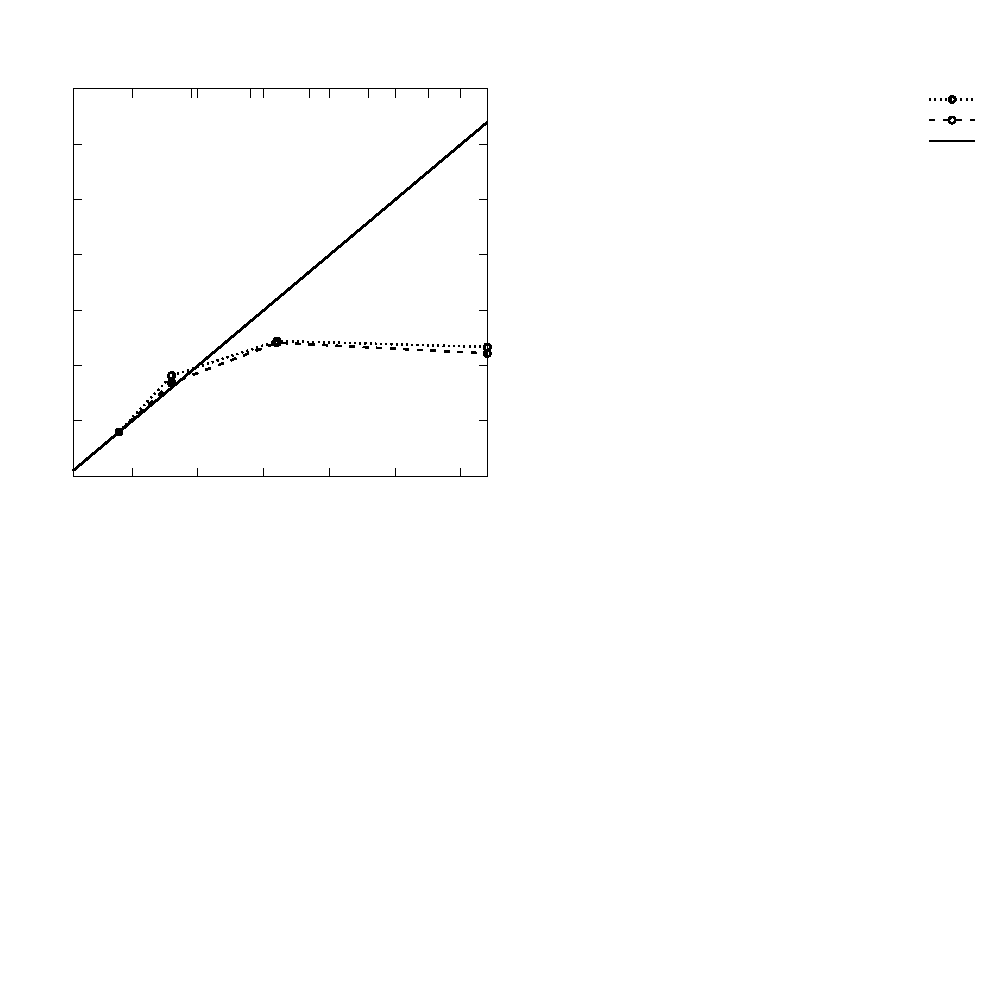
\includegraphics{Additional_2}}%
    \gplfronttext
  \end{picture}%
\endgroup
